\subsection{Implementando traceroute}

Como dijimos anteriormente, \emph{traceroute} es una herramienta de dign\'ostico que se utiliza para hacer
un an\'alisis del estado de la conexi\'on entre 2 hosts comunicados a trav\'es del protocolo TCP/IP.
Este comando pone especial \'enfasis en los distintos tramos (determinados por los hops entre routers)
que va debe atravesar el paquete para llegar a destino.
Mediante este tipo de an\'alisis es posible obtener informaci\'on de gran inter\'es, como por
ejemplo identificar los enlaces con mayor RTT (determinantes en el c\'alculo del
RTT ''global'', entre el host origen y el destino). De esta manera es posible caracterizar los distintos
enlaces: RTT's altos pueden corresponderse a enlaces submarinos o terrestres de largas distancias, o
enlaces con poca velocidad de transmisi\'on.

La idea b\'asica del algoritmo consiste en enviar paquetes con TTL's incrementales hacia el nodo destino
y obtener informaci\'on en funci\'on de los datagramas ICMP obtenidos, tal como muestra el siguiente
diagrama:

\begin{figure}[!h]
  \begin{center}
      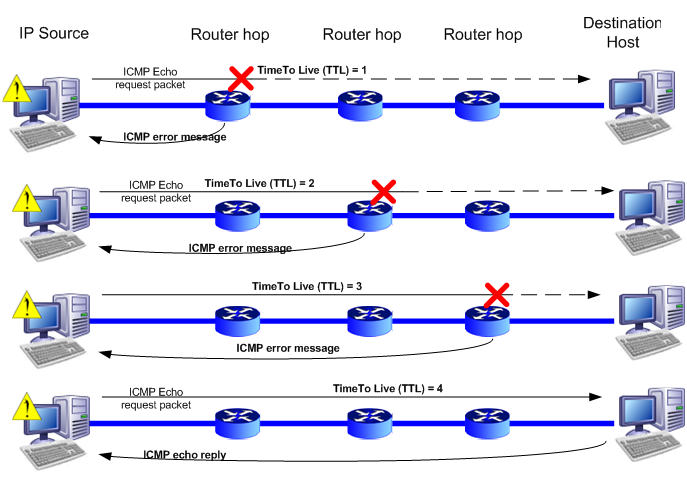
\includegraphics[scale=0.4]{imagenes/traceroute.png}
      \caption{Mecanismo de acci\'on de traceroute}
      \label{fig:contra1}
  \end{center}
\end{figure}

Cada vez que un paquete es forwardeado hacia un router, el valor de su TTL se decrementa en una unidad.
Cuando un routers advierte que el TTL de un paquete ha alcanzado el valor 0, env\'ia un mensaje ICMP hacia
el host fuente del mensaje, de tipo ''time exceeded''. Conociendo la hora exacta de emisi\'on del paquete
original y hora en la cual arriba el mensaje de error es posible determinar el RTT entre el host en el cual se corre el algoritmo
y el router generador del paquete ICMP.
El algoritmo se extiende a cada uno de los nodos intermedios:
En la primera iteraci\'on se env\'ia un paquete con valor de TTL 1. Por lo tanto el router a 1 hop de
distancia env\'ia un mensaje de error, y el algoritmo puede calcular el RTT entre el origen y dicho
router.
Generalizando, en la iteraci\'on $i$ se env\'ia un paquete con valor de TTL $i$, y utilizando la informaci\'on
recibida, el algoritmo puede calcular el RTT entre el origen y el router ubicado a $i$ hops.
El algoritmo finaliza o bien cuando se recibe una respuesta afirmativa por parte del destino; o bien
cuando se alcanza el l\'imite de TTL permitido.

\subsubsection{Algunas consideraciones y detalles implementativos}

Para implementar el comando utilizamos la librer\'ia \emph{Scapy} de Python.

Traceroute por default env\'ia una secuencia de paquetes UDP hacia el nodo destino. Paquetes del estilo
TCP SYN tambi\'en pueden ser usados. En nuestra implementaci\'on la alternativa utilizada son los paquetes
ICMP de tipo ''echo request'' . Los mensajes recibidos ser\'an por lo tanto del tipo ''time exceeded''
para los nodos intermedios y ''echo reply'' cuando el paquete llega a destino.

La funci\'on debe recibir como argumentos el valor de TTL inicial con el que env\'ia el primer paquete
y el m\'aximo de saltos permitidos hasta alcanzar el destino. En nuestro caso utilizamos los valores
por defecto: 1 y 30 respectivamente.

Otro de los par\'ametros que debe especificarse es el n\'umero de reintentos que debe realizarse por cada
valor de TTL. ICMP, al igual que IP, es una capa ''sin garant\'ias'' en el env\'io de mensajes. Los routers
hacen el ''mejor esfuerzo'' para lograr el env\'io de los paquetes, pero no hay garant\'ias de que los mismos
alcancen el destino.
Teniendo esto en cuenta, es posible que los mensajes ICMP enviados por los routers no lleguen al emisor.
En dicho caso, es deseable que se realice m\'as de un intento para un determinado valor de TTL.
Usualmente la mayor\'ia de las implmentaciones utilizan 2 o 3 como valor. En nuestro caso decidimos
realizar 10 intentos por cada TTL. Este valor nos protege contra otro aspecto sensible del algoritmo,
descripto a continuaci\'on.

Un paquete no llega al mismo destino atravesando siempre las mismas rutas. Los nodos intermedios pueden
caerse o levantarse. Determinados enlaces pueden congestionarse o liberarse en distintos momentos.
Supongamos que el algoritmo env\'ia hacia el destino un paquete con TTL 10. ?`Qu\'e garant\'ias tenemos de que,
en caso de ser necesario un segundo intento porque no ha llegado ning\'un mensaje de error, el router
alcanzado luego del d\'ecimo hop sea el mismo? Ninguna. En otras palabras, dependiendo la ruta que siga
el datagrama, el router alcanzado luego del d\'ecimo hop ser\'a uno u otro.
Para tener cierto control respecto a esta situaci\'on, por cada valor de TTL se env\'ian 10 paquetes y
se guardan todas las direcciones de IP que han respondido los mensajes de error.
Luego, el algoritmo selecciona aquella direcci\'on que ha respondido m\'as veces.

Finalmente, el valor de RTT entre el host que corre el \emph{traceroute} y el router a $i$ hops de
distancia es calculado como el promedio de los valores obtenidos por cada intento.


\subsection{Estimando Enlaces Intercontinentals}

Recordando algunas f\'ormulas pertenecientes a la capa de enlace, sabemos que el delay est\'a determinado
por la siguiente ecuaci\'on:

~

$delay[seg] = T_{tx} + T_{prop}$, donde $T_{tx}$ es el tiempo de transmisi\'on determinado principalmente
por la capacidad del canal y la relaci\'on se\~nal ruido dentro del mismo, y el tiempo de propagaci\'on
est\'a determinado por:

~

$T_{prop} = \frac{D}{V}$, con $D$ la distancia del enlace y $V$ la velocidad de propagaci\'on de la forma
de onda en el medio f\'isico.

~

El RTT equivale a $2*delay$.

~

Si analizamos exclusivamente la capa de enlace punto a punto del modelo de capas de Internet, podemos
llegar a la conclusi\'on de que el factor de mayor peso en el c\'alculo del RTT es la distancia del enlace.
Dado que se env\'ia un \'unico datagrama con una cantidad despreciable de datos de test (caracteres
ASCII pertenecientes al ''echo request''), el tiempo de transmisi\'on del mismo dentro del enlace es
\'infimo (independientemente de la velocidad de transmisi\'on de dicho enlace). Por lo tanto, desde este
punto de vista es l\'ogico pensar que los resultados con mayor valor de RTT corresponder\'an a enlaces
submarinos. Suponemos que el tiempo que le toma a un paquete ir de un nodo a otro
por tierra es significativamente menor al que le toma atravesar un
enlace intercontinental, ya que estos \'ultimos cubren distancias mucho mayores.

Sin embargo, la capa de nivel 1 no es la \'unica que debemos tener en cuenta a la hora de realizar el
an\'alisis. Podr\'ia suceder que por alg\'un motivo (congesti\'on, por ejemplo), el paquete sea almacenado
temporalmente en un buffer antes de ser forwardeado hacia el pr\'oximo router. O que alg\'un conflicto
de \'indole similar suceda a nivel Ethernet. Por lo tanto, estos factores pueden influir
en un resultado con RTT alto sin que el router involucrado provenga necesariamente de un enlace
submarino.

~

El \emph{zscore} es una medida que nos permite medir el peso de un hop respecto a los dem\'as. (En
particular, respecto a la media de todos los hops de la ruta, y considerando tambi\'en el desv\'io
standard de los datos).
La f\'ormula utilizada para calcularlo es:

~

$ZRTT_{i} = \frac{RTT_{i} - RTT_{mean}}{SRTT}$

~

$ZRTT_{i}$ representa el RTT para el i-\'esimo hop. Para calcularlo, obtenemos la distancia en tiempo
que hay entre los pares de nodos vecinos y asumimos que los
mismos siguen una distribuci\'on normal.
Finalmente fijamos un umbral de Zscore para determinar los tramos
son submarinos.
